% =========================================================================
% Recap del paper rifiutato (IEEE TCSS)
% "From Articles to Publishers". Solo recap di cosa e' stato fatto;
% le review si vedono nei messaggi successivi.
% Stile Madrid, poche voci per slide, una alla volta, con qualche figura.
% La parte statistica (chi-quadro) e' spiegata passo passo in modo semplice.
% Build: tectonic recap_paper.tex
% =========================================================================
\documentclass[aspectratio=169]{beamer}
\usetheme{Madrid}
\usecolortheme{whale}
\usepackage[T1]{fontenc}
\usepackage{graphicx}
\usepackage{booktabs}
\usepackage{xcolor}
\graphicspath{{../Paper/OldPaperRejected/img/}}

\beamertemplatenavigationsymbolsempty
\setbeamercovered{transparent}
\setbeamertemplate{caption}{\insertcaption}
\newcommand{\hl}[1]{\textbf{#1}}
\definecolor{wrongred}{RGB}{176,0,32}
\newcommand{\wrong}[1]{\textcolor{wrongred}{#1}}

\title[Verso Web Science 2027]{Verso Web Science 2027}
\subtitle{Riprendere il paper bocciato: recap del lavoro e prossimi passi}
\author[Riunione di gruppo]{Riunione di gruppo}
\institute[]{IMT Lucca \& IIT-CNR Pisa}
\date{}

\begin{document}

% ---------------------------------------------------------------- titolo
\begin{frame}
  \titlepage
\end{frame}

% ---------------------------------------------------------------- divider: recap
\begin{frame}[plain]
  \vfill
  \begin{center}
    {\usebeamercolor[fg]{title}\Large\textbf{Parte 1 --- Recap del paper}}\\[0.8em]
    \normalsize \textbf{Recap del paper bocciato} (non della versione sottomessa ad IR FOR GOOD)\\[0.3em]
  \end{center}
  \vfill
\end{frame}

% ---------------------------------------------------------------- dati
\begin{frame}{Dati}
  \begin{columns}[c]
    \begin{column}{0.52\textwidth}
      \begin{itemize}[<+->]
        \setlength\itemsep{0.8em}
        \item Scraping con \hl{newspaper3k}
        \item 439 editori, 19.476 articoli politici in inglese
        \item Etichette \hl{NewsGuard}: 5 livelli $l_1$--$l_5$ (da 0--100)
        \item Ogni articolo \hl{eredita} l'etichetta del suo editore
      \end{itemize}
    \end{column}
    \begin{column}{0.48\textwidth}
      \onslide<3->{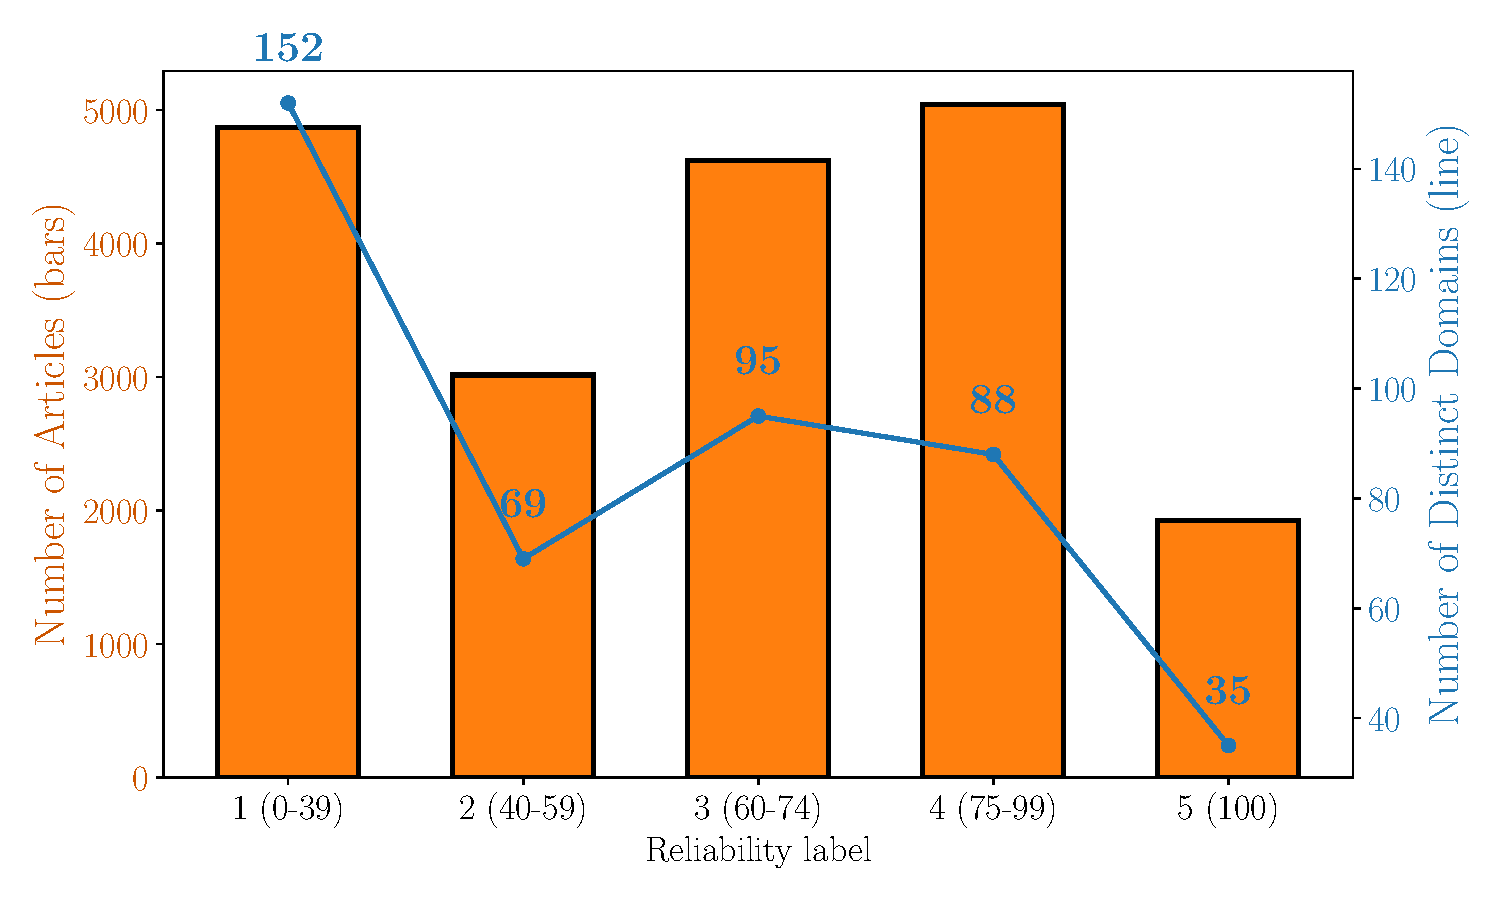
\includegraphics[width=\linewidth]{dataset_distribution.pdf}}
    \end{column}
  \end{columns}
\end{frame}

% ---------------------------------------------------------------- classificazione
\begin{frame}{Classificazione --- livello articolo}
  \begin{columns}[c]
    \begin{column}{0.5\textwidth}
      \begin{itemize}[<+->]
        \setlength\itemsep{0.8em}
        \item Quattro transformer: \hl{BERT, RoBERTa, Llama, Mistral}
        \item Encoder full fine-tuning, decoder con \hl{LoRA}
        \item Input \hl{256 token} (1024 per Mistral)
        \item Split \hl{publisher-disjoint}: editori di test mai visti
      \end{itemize}
    \end{column}
    \begin{column}{0.5\textwidth}
      \onslide<5->{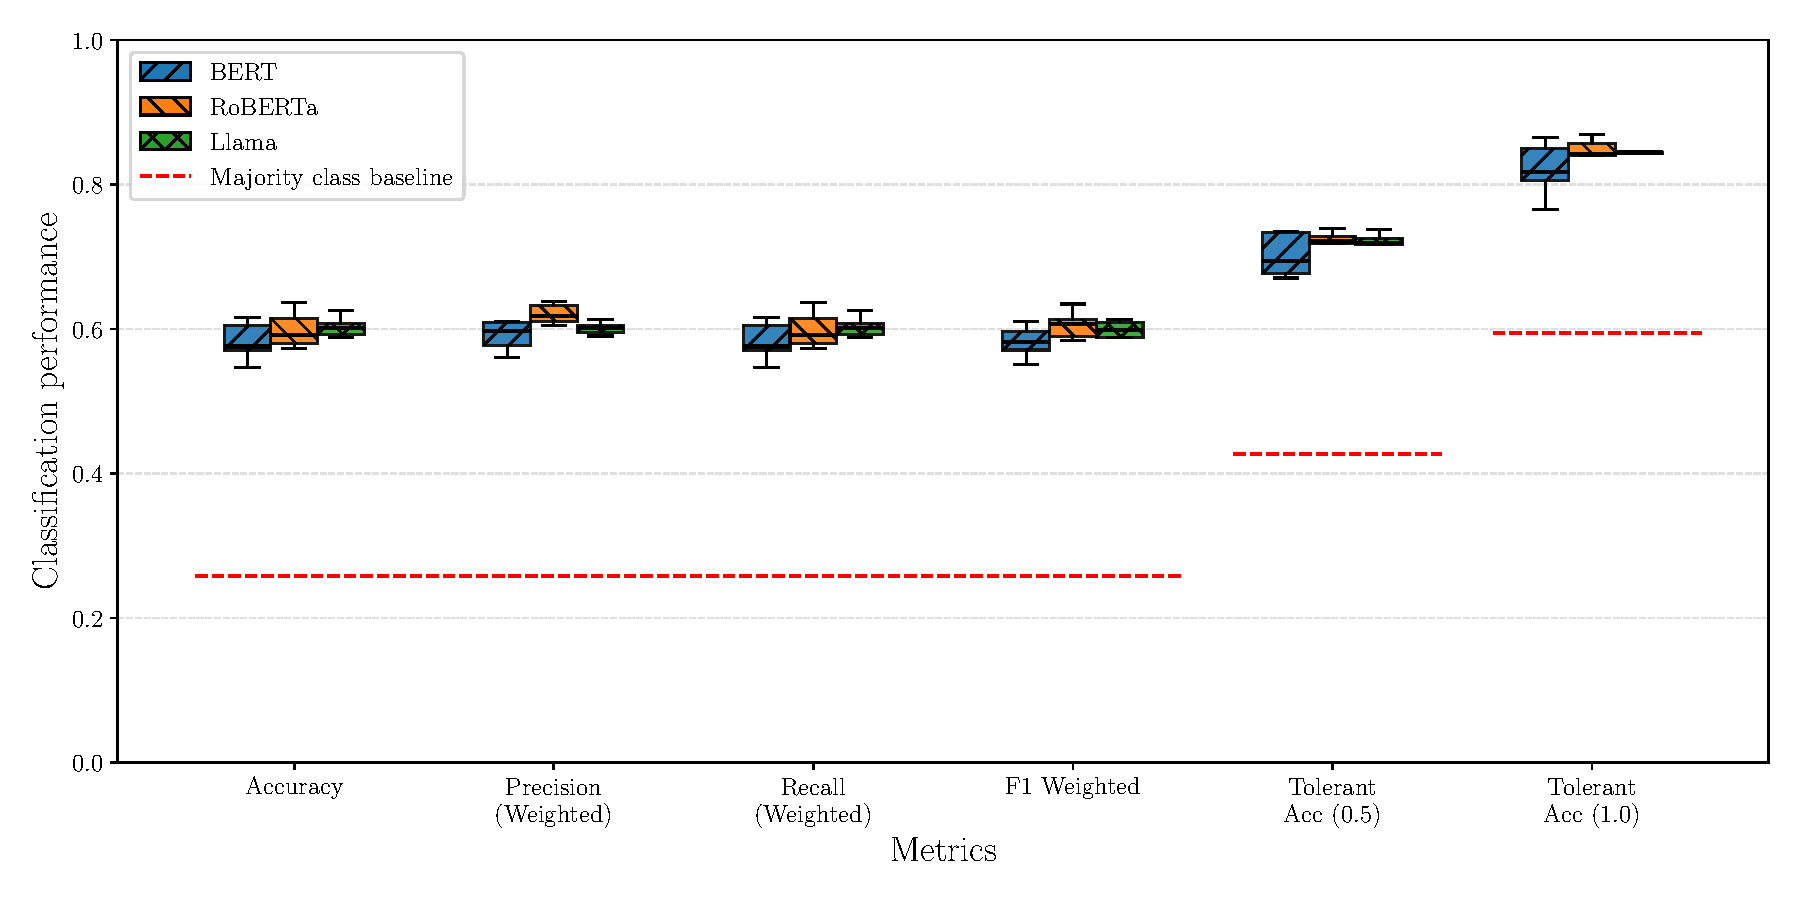
\includegraphics[width=\linewidth]{results_boxplot_baselines.pdf}}
    \end{column}
  \end{columns}
\end{frame}

% ---------------------------------------------------------------- aggregazione
\begin{frame}{Aggregazione --- livello editore}
  \begin{columns}[c]
    \begin{column}{0.5\textwidth}
      \begin{itemize}[<+->]
        \setlength\itemsep{0.9em}
        \item Dall'articolo all'editore con \hl{majority voting}
        \item Si combina il voto di tutti gli articoli dell'editore
        \item Valutazione su editori \hl{mai visti} in addestramento
      \end{itemize}
    \end{column}
    \begin{column}{0.5\textwidth}
      \onslide<4->{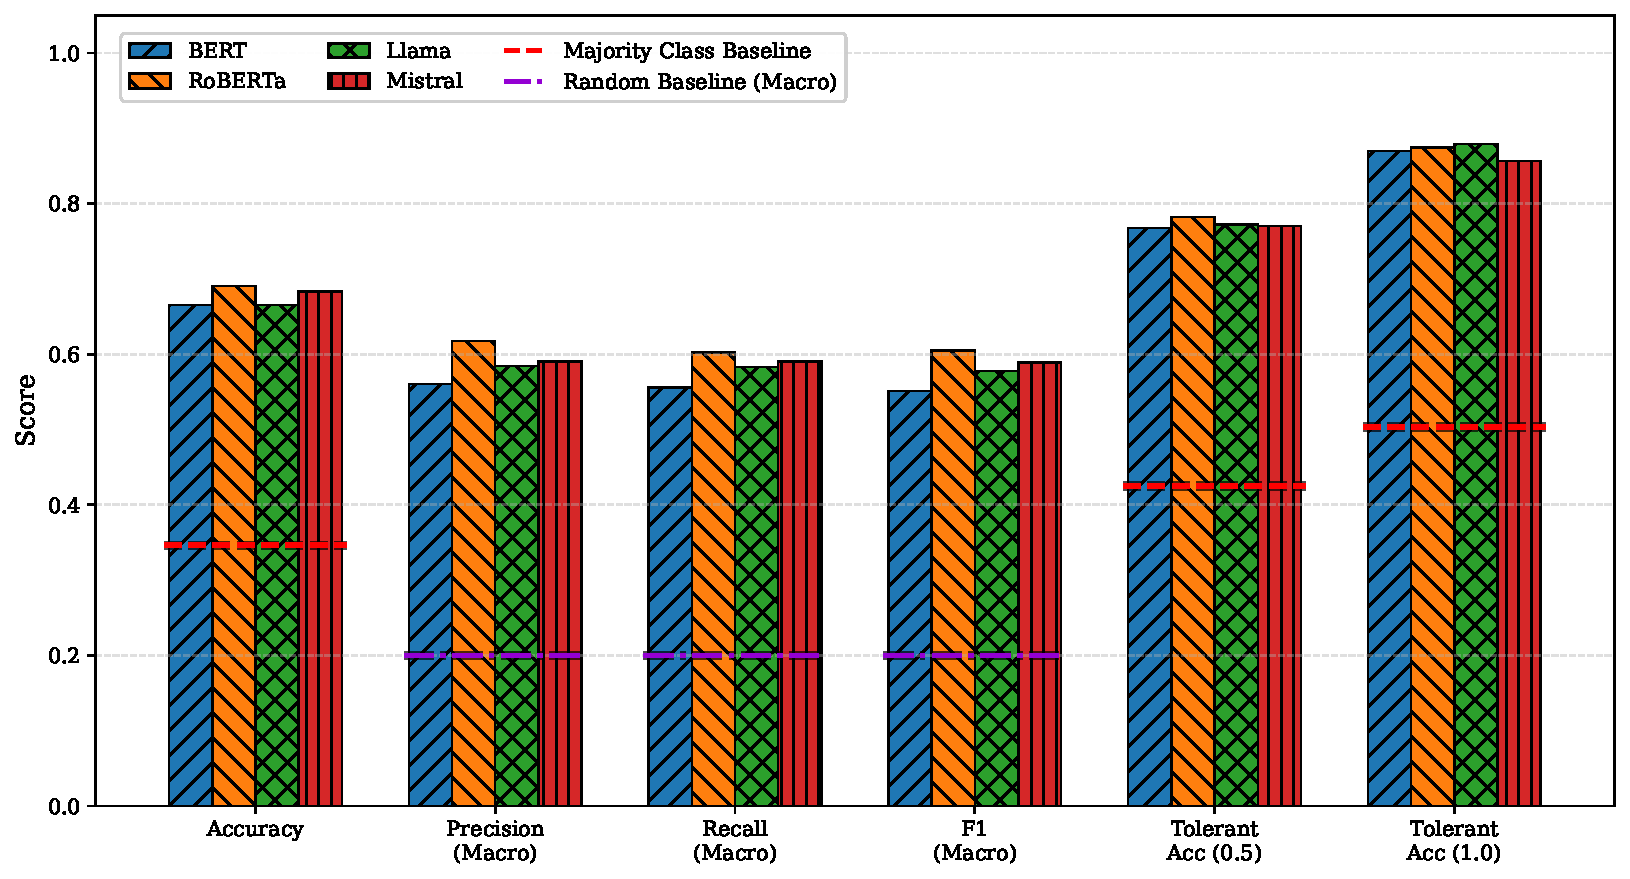
\includegraphics[width=\linewidth]{domain_metrics_comparison.pdf}}
    \end{column}
  \end{columns}
\end{frame}

% ================================================================
%  ANALISI DELL'ERRORE (livello di affidabilita')
% ================================================================

% ---------------------------------------------------------------- motivazione errore
\begin{frame}{Perch\'e analizziamo gli errori}
  \vfill
  \begin{itemize}[<+->]
    \setlength\itemsep{0.9em}
    \item Oltre alle metriche aggregate, vogliamo capire \hl{come} e \hl{perch\'e} i modelli sbagliano
    \item[] {\small\itshape ``Beyond aggregate performance, we investigate how and why models fail.''}
    \item Obiettivo: trovare \hl{debolezze strutturali} --- su quali livelli sbaglia e se sovra/sottostima
    \item[] {\small\itshape ``To detect structural weaknesses\dots''}
  \end{itemize}
  \vfill
\end{frame}

% ---------------------------------------------------------------- errore: per livello
\begin{frame}{Analisi dell'errore --- per livello}
  \begin{columns}[c]
    \begin{column}{0.5\textwidth}
      \begin{itemize}[<+->]
        \setlength\itemsep{0.9em}
        \item \hl{Error rate} per ogni livello di affidabilit\`a
        \item $l_1$ il pi\`u \hl{facile}: contenuti molto inaffidabili riconoscibili
        \item $l_5$ il pi\`u \hl{difficile}: si confonde con $l_4$
        \item $l_2$ difficile, $l_3$ intermedio
      \end{itemize}
    \end{column}
    \begin{column}{0.5\textwidth}
      \onslide<2->{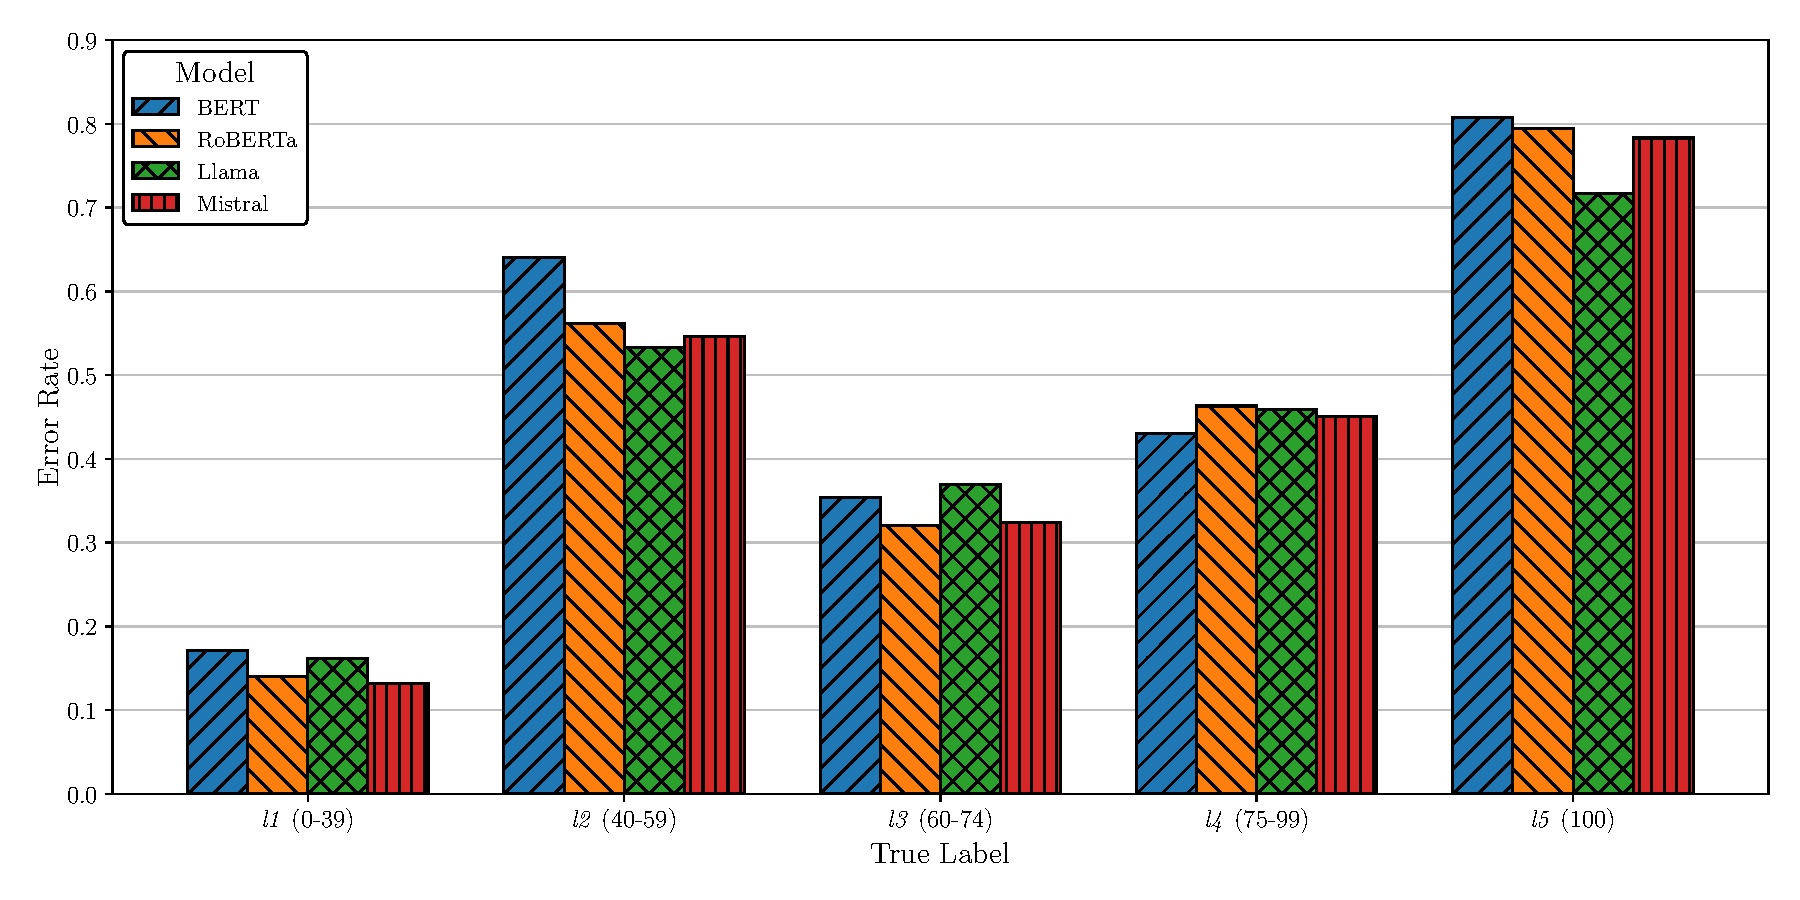
\includegraphics[width=\linewidth]{error_rate_analysis.pdf}}
    \end{column}
  \end{columns}
\end{frame}

% ---------------------------------------------------------------- errore: direzione per livello
\begin{frame}{Analisi dell'errore --- direzione}
  \begin{columns}[c]
    \begin{column}{0.5\textwidth}
      \begin{itemize}[<+->]
        \setlength\itemsep{0.9em}
        \item \hl{Mean Error Direction}: l'errore \emph{sovrastima} ($+$) o \emph{sottostima} ($-$) l'affidabilit\`a
        \item Livelli \hl{bassi sovrastimati}, livelli \hl{alti sottostimati}
        \item Gli errori ``tirano verso il \hl{centro}'' della scala
      \end{itemize}
    \end{column}
    \begin{column}{0.5\textwidth}
      \onslide<2->{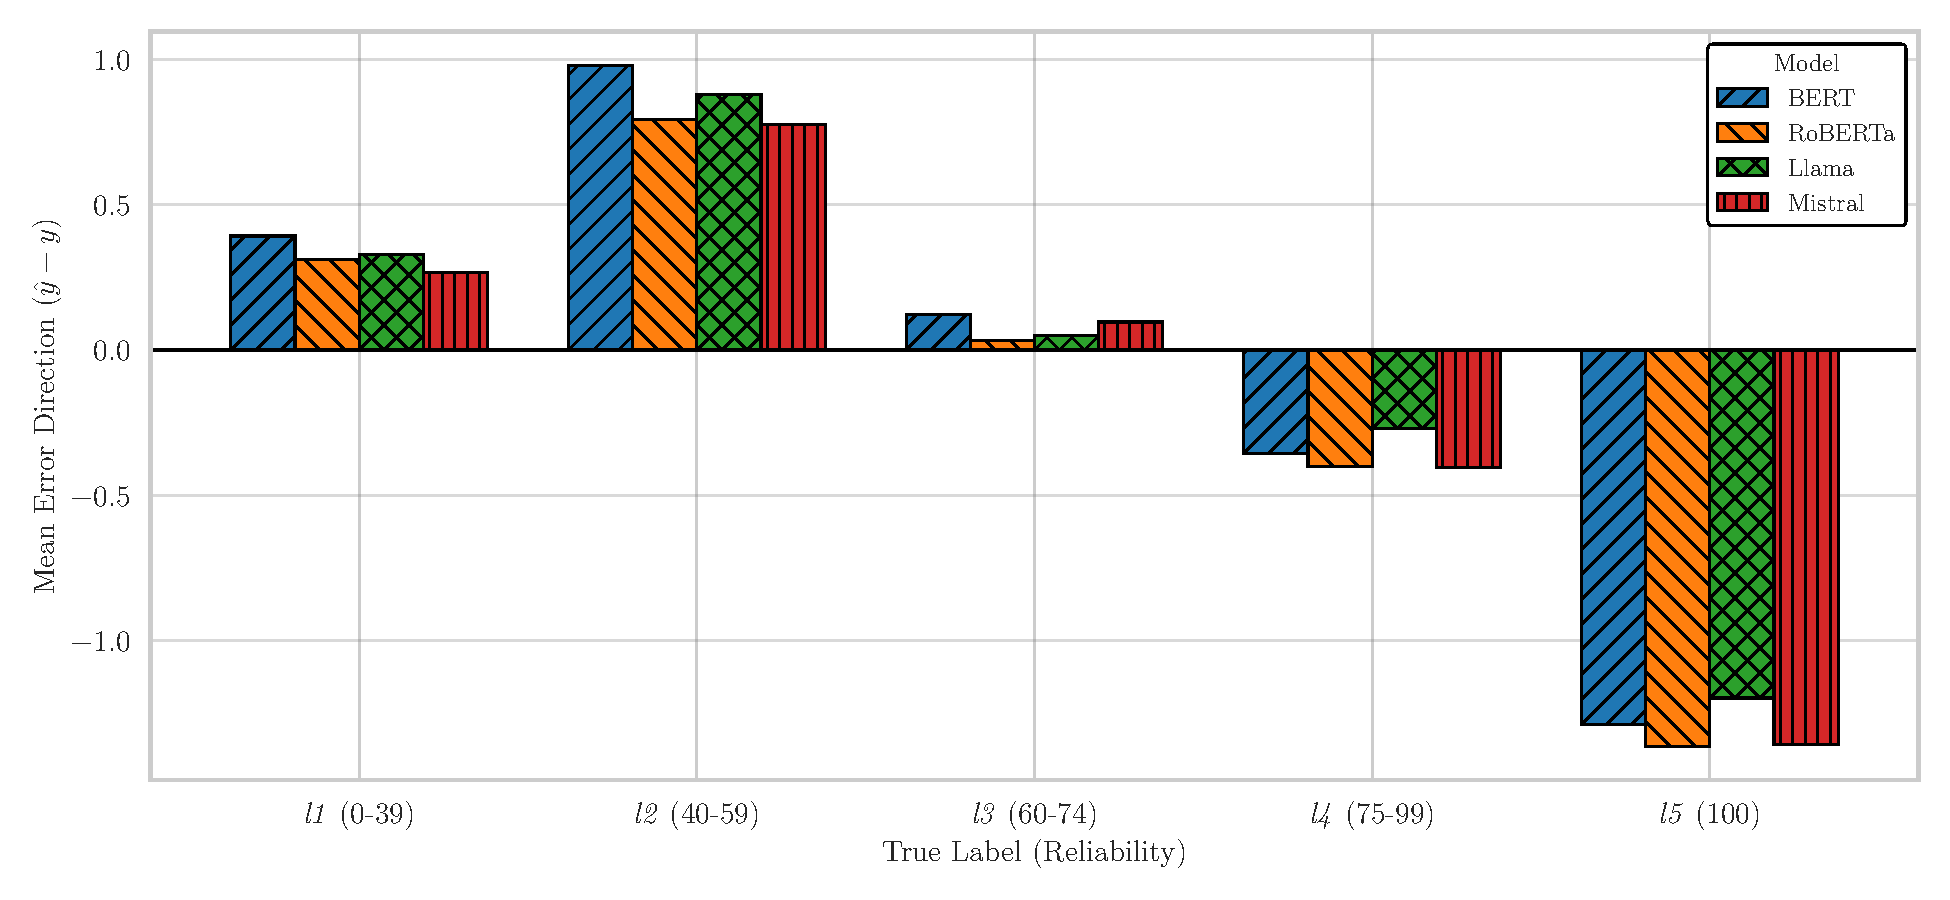
\includegraphics[width=\linewidth]{mean_error_direction.pdf}}
    \end{column}
  \end{columns}
\end{frame}

% ================================================================
%  ANALISI DEGLI ERRORI PER BIAS POLITICO
% ================================================================

% ---------------------------------------------------------------- motivazione bias
\begin{frame}{Perch\'e analizziamo il bias politico}
  \vfill
  \begin{itemize}[<+->]
    \setlength\itemsep{0.9em}
    \item Vogliamo sapere se il modello \hl{tratta allo stesso modo} tutto lo spettro politico, o se \hl{penalizza} certi orientamenti
    \item[] {\small\itshape ``\dots determine if the models exhibit political bias\dots whether the models treat all sides of the political spectrum equally or if they penalize specific orientations.''}
    \item Serve una valutazione \hl{bias-aware}: un sistema in uso con bias politico pu\`o fare danni
    \item[] {\small\itshape ``\dots the need for bias-aware evaluation protocols\dots''}
  \end{itemize}
  \vfill
\end{frame}

% ---------------------------------------------------------------- bias: distribuzione
\begin{frame}{Bias politico --- distribuzione dei dati}
  \begin{columns}[c]
    \begin{column}{0.5\textwidth}
      \begin{itemize}[<+->]
        \setlength\itemsep{0.9em}
        \item Orientamento ereditato dall'editore (analisi \emph{a posteriori})
        \item Dentro ogni orientamento, come si distribuiscono i livelli
        \item Distribuzione molto \hl{sbilanciata} (propriet\`a del sistema mediatico)
        \item Per questo gli error rate si calcolano \hl{classe per classe}
      \end{itemize}
    \end{column}
    \begin{column}{0.5\textwidth}
      \onslide<2->{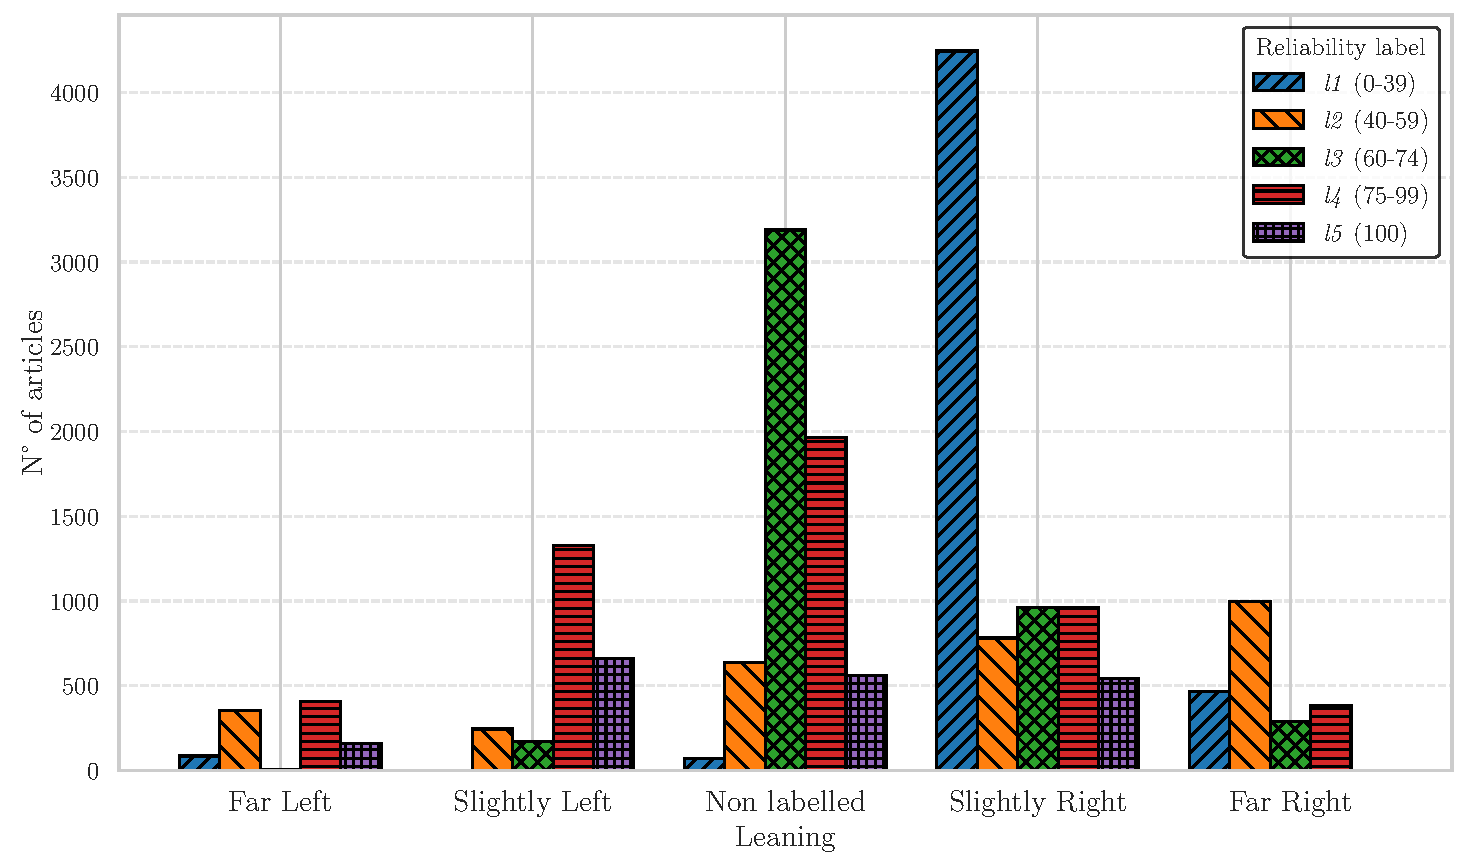
\includegraphics[width=\linewidth]{orientationDistributionInverted.pdf}}
    \end{column}
  \end{columns}
\end{frame}

% ---------------------------------------------------------------- bias: error rate
\begin{frame}{Bias politico --- error rate}
  \begin{columns}[c]
    \begin{column}{0.5\textwidth}
      \begin{itemize}[<+->]
        \setlength\itemsep{0.9em}
        \item \hl{Error rate} per orientamento politico
        \item Gli estremi (\hl{far left}, \hl{far right}) sbagliano molto di pi\`u
        \item Slightly right e non labelled i pi\`u \hl{facili}
      \end{itemize}
    \end{column}
    \begin{column}{0.5\textwidth}
      \onslide<2->{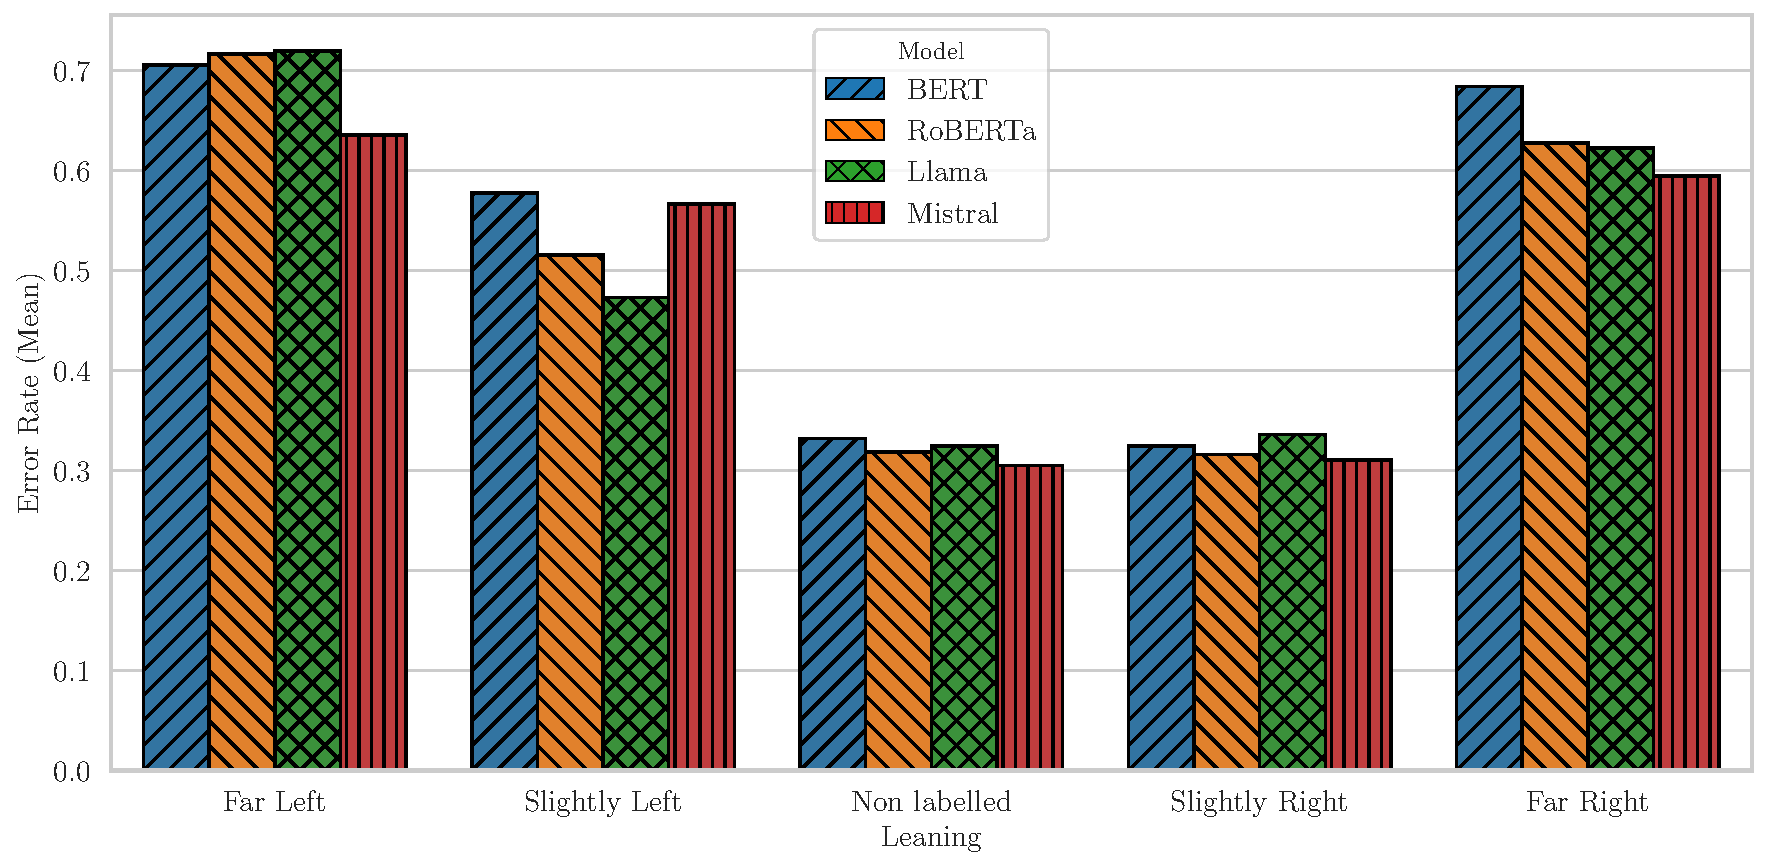
\includegraphics[width=\linewidth]{politicalErrorRates.pdf}}
    \end{column}
  \end{columns}
\end{frame}

% ---------------------------------------------------------------- bias: direzione
\begin{frame}{Bias politico --- direzione dell'errore}
  \begin{columns}[c]
    \begin{column}{0.5\textwidth}
      \begin{itemize}[<+->]
        \setlength\itemsep{0.9em}
        \item \hl{Mean Error Direction} per orientamento
        \item Estremi (far left, far right) \hl{sovrastimati}
        \item Slightly left \hl{sottostimato}
        \item Slightly right e non labelled: deviazioni piccole
      \end{itemize}
    \end{column}
    \begin{column}{0.5\textwidth}
      \onslide<2->{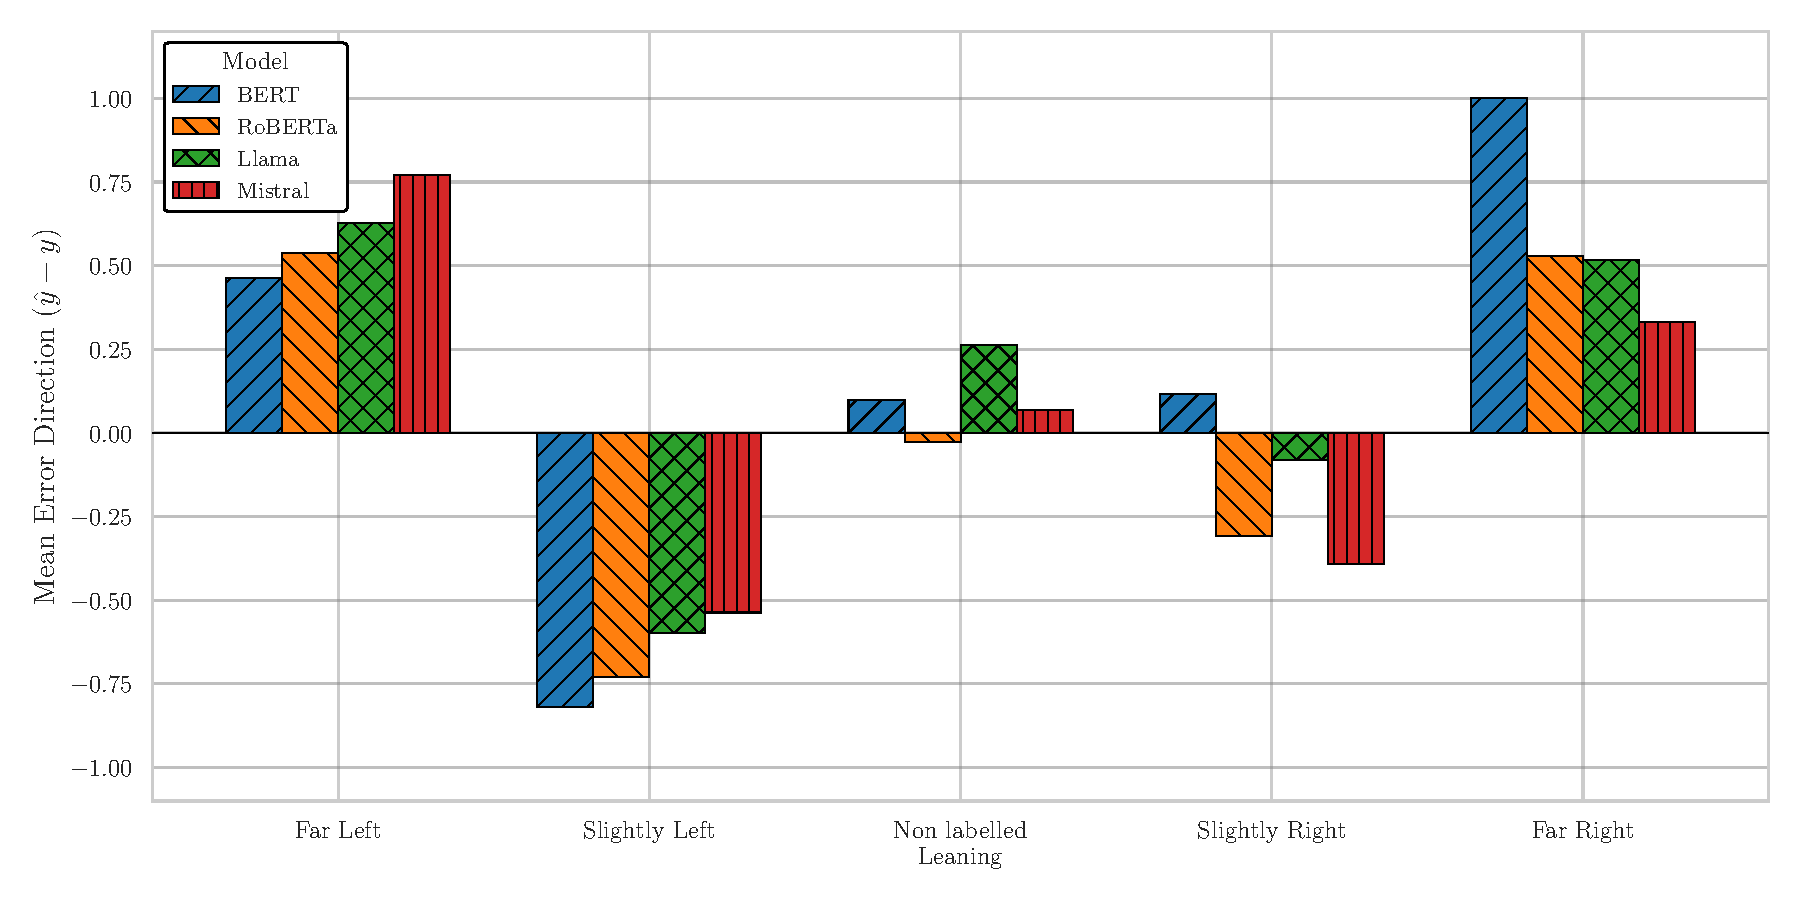
\includegraphics[width=\linewidth]{politicalErrorsDirection.pdf}}
    \end{column}
  \end{columns}
\end{frame}

% ---------------------------------------------------------------- stat: la domanda
\begin{frame}{\`E un vero legame o \`e un caso?}
  \vfill
  \begin{itemize}[<+->]
    \setlength\itemsep{1.0em}
    \item Vediamo error rate diversi tra gli orientamenti.
    \item Ma potrebbe essere solo \hl{rumore} dei dati.
    \item Serve un \hl{test statistico} che dica: questo legame \`e reale?
  \end{itemize}
  \vfill
  \onslide<4->{\begin{center}\small Strumento usato: il \hl{test del chi-quadro ($\chi^2$) di indipendenza}.\end{center}}
\end{frame}

% ---------------------------------------------------------------- stat: tabella contingenza
\begin{frame}{Passo 1 --- mettiamo gli errori in tabella}
  \begin{columns}[c]
    \begin{column}{0.46\textwidth}
      \begin{itemize}[<+->]
        \setlength\itemsep{0.8em}
        \item Per ogni orientamento contiamo \hl{giusti} e \hl{sbagliati}
        \item \`E la \hl{tabella di contingenza}
        \item Agli estremi gli \wrong{sbagliati} superano i giusti
      \end{itemize}
    \end{column}
    \begin{column}{0.54\textwidth}
      \onslide<2->{%
      \footnotesize
      \begin{center}
      \begin{tabular}{lrr}
        \toprule
        \textbf{Orientamento} & \textbf{Giusti} & \textbf{\wrong{Sbagliati}} \\
        \midrule
        Far Left       & 299  & \wrong{716}  \\
        Slightly Left  & 1018 & \wrong{1389} \\
        Non labelled   & 4292 & 2130 \\
        Slightly Right & 5062 & 2428 \\
        Far Right      & 678  & \wrong{1464} \\
        \bottomrule
      \end{tabular}
      \end{center}
      \scriptsize\centering (esempio: BERT)
      }
    \end{column}
  \end{columns}
\end{frame}

% ---------------------------------------------------------------- stat: idea del chi2
\begin{frame}{Passo 2 --- l'idea del chi-quadro}
  \vfill
  \begin{itemize}[<+->]
    \setlength\itemsep{0.9em}
    \item Immaginiamo che l'orientamento \hl{non c'entri} con gli errori.
    \item Allora ogni gruppo dovrebbe sbagliare \hl{nella stessa proporzione} (circa la media, $\sim$42\%).
    \item Il $\chi^2$ misura \hl{quanto} gli errori \emph{osservati} si allontanano da questo scenario ``senza legame''.
    \item Pi\`u grande \`e lo scarto $\rightarrow$ $\chi^2$ grande $\rightarrow$ pi\`u probabile che un legame ci sia.
  \end{itemize}
  \vfill
\end{frame}

% ---------------------------------------------------------------- stat: p-value
\begin{frame}{Passo 3 --- il $p$-value}
  \vfill
  \begin{itemize}[<+->]
    \setlength\itemsep{0.9em}
    \item Un $\chi^2$ grande potrebbe capitare \hl{per caso}?
    \item Il \hl{$p$-value} \`e la probabilit\`a di vedere uno scarto cos\`i grande \emph{se non ci fosse nessun legame}.
    \item $p$ piccolissimo (es. $p<0.001$) $\rightarrow$ quasi impossibile che sia un caso.
    \item Quindi il legame \`e \hl{reale}, non fortuna.
  \end{itemize}
  \vfill
\end{frame}

% ---------------------------------------------------------------- stat: Cramer V
\begin{frame}{Passo 4 --- quanto \`e forte? (Cram\'er's V)}
  \vfill
  \begin{itemize}[<+->]
    \setlength\itemsep{0.9em}
    \item Il $p$-value dice \hl{se} c'\`e un legame, non \hl{quanto} \`e forte.
    \item Con tanti dati anche un legame \hl{piccolo} risulta ``significativo''.
    \item \hl{Cram\'er's V} misura la \hl{forza}: 0 = nessun legame, 1 = legame massimo.
  \end{itemize}
  \vfill
\end{frame}

% ---------------------------------------------------------------- stat: sintesi + tabella
\begin{frame}{In sintesi}
  \begin{columns}[c]
    \begin{column}{0.46\textwidth}
      \begin{itemize}[<+->]
        \setlength\itemsep{0.9em}
        \item Legame \hl{statisticamente significativo} (tutti i modelli)
        \item Forza \hl{piccola--moderata} (V $\approx$ 0.25--0.29)
        \item Direzione: estremi \hl{sovrastimati}, slightly left \hl{sottostimati}
      \end{itemize}
    \end{column}
    \begin{column}{0.54\textwidth}
      \onslide<2->{%
      \footnotesize
      \begin{center}
      \begin{tabular}{lrcc}
        \toprule
        \textbf{Model} & $\boldsymbol{\chi^2}$ & \textbf{$p$} & \textbf{V} \\
        \midrule
        BERT    & 1684 & $<10^{-300}$ & 0.294 \\
        RoBERTa & 1418 & $<10^{-300}$ & 0.270 \\
        Llama   & 1208 & $<10^{-250}$ & 0.249 \\
        Mistral & 1344 & $<10^{-300}$ & 0.263 \\
        \bottomrule
      \end{tabular}
      \end{center}}
    \end{column}
  \end{columns}
\end{frame}

% ---------------------------------------------------------------- supplementary
\begin{frame}{Nel materiale supplementare}
  \vfill
  \begin{itemize}[<+->]
    \setlength\itemsep{0.9em}
    \item Matrici di confusione per \hl{fold} (livello articolo)
    \item Matrici di confusione a \hl{livello editore} (dopo aggregazione)
    \item Matrici di confusione per \hl{orientamento politico}
    \item \hl{Analisi di convergenza}: curve di loss (Llama, Mistral)
  \end{itemize}
  \vfill
  \onslide<5->{\begin{center}\small Dettagli a supporto delle analisi del paper, non nuovi risultati.\end{center}}
\end{frame}

% ---------------------------------------------------------------- chiusura
\begin{frame}[plain]
  \vfill
  \begin{center}
    {\usebeamercolor[fg]{title}\large Prossimo passo: le \textbf{review}}
  \end{center}
  \vfill
\end{frame}

\end{document}
